\documentclass{article}
\usepackage{graphicx} % Required for inserting images
\usepackage{amsmath}
\usepackage{comment}
\usepackage[final]{project_440_550}

% Please submit it as is here, with line numbers.
% If you'd like a "less draft"-looking version for your website or something after:
%     \usepackage[final]{project_440_550}   % keeps the footer but kills line numbers,
%     \usepackage[preprint]{project_440_550}   % removes both

\usepackage[utf8]{inputenc} % allow utf-8 input
\usepackage[T1]{fontenc}    % use 8-bit T1 fonts

\usepackage[USenglish]{babel}  % there's a "canadian" option, but it's an alias for USenglish,
                               % and for some reason it makes csqoutes behave differently...
\usepackage{csquotes}       % smarter handling of quotes (used by biblatex)

\usepackage{booktabs}       % professional-quality tables
\usepackage{amsfonts}       % blackboard math symbols
\usepackage{nicefrac}       % compact symbols for 1/2, etc.
\usepackage{microtype}      % microtypography
\usepackage{xcolor}         % colors
\usepackage{hyperref}       % hyperlinks
\usepackage{url}            % simple URL typesetting

% I recommend the biblatex package.
% If you hate it for some reason, though, you can use natbib instead:
% comment out this block and uncomment the next one.

\usepackage[style=authoryear,maxbibnames=30,natbib]{biblatex}
\addbibresource{refs.bib}
\renewbibmacro{in:}{}  % drops a silly "In:" from biblatex format
\DeclareDelimFormat{nameyeardelim}{\addspace} % remove a comma i dislike, doesn't matter
\DeclareNameAlias{sortname}{given-family}  % avoid kinda-weird bib printing order

%\usepackage[round]{natbib}
%\newcommand{\printbibliography}{\bibliographystyle{plainnat}\bibliography{refs}}


\usepackage[capitalize,noabbrev]{cleveref}

\title{A Bayesian Approach to In-Game Win Probability in the NHL}
\author{%
  Daniel Kaichis\\
  \texttt{dk44@rogers.com}
  \And
  Oscar Poitras\\
  \texttt{oscar.poitras10@gmail.com}
}
\date{April 2026}

\begin{document}

\maketitle

\begin{abstract}
Existing in-game win probability models for the NHL rely on fixed league-wide scoring rates without team-specific information. We propose a Bayesian framework that conditions Poisson scoring rates on the current manpower state, incorporates team-specific offensive and defensive strength through a hierarchical prior, and estimates win probabilities via Monte Carlo simulation over the posterior predictive distribution. We evaluated three variants on NHL play-by-play data from the 2023-2025 seasons across in-game checkpoints from 50 to 2 minutes remaining. Our sequential model, updated in rolling 20-day windows, achieves Brier scores below 0.18 and accuracy between 70\% and 86\% at all checkpoints from 20 to 50 minutes remaining, consistently outperforming both our league-wide baseline model and the pre-game moneyline betting-favourite accuracy of 55.7\%.
\end{abstract}


\section{Introduction}

Predicting the outcome of sports games using statistical models has been an active area of research for decades, but most prior work focuses on pre-game prediction rather than in-game win probabilities. Live win probability has value as a "story stat" for fan engagement, for evaluating in-game decision-making via win probability added (WPA), and for in-game betting \citep{robberechts2021bayesian}. While in-game win probability models exist for the NHL \citep{pettigrew2015assessing}, they rely on fixed league-wide scoring rates with no team-specific information and no uncertainty quantification.


We draw on the generative Bayesian approach of \citet{robberechts2021bayesian}, who model future goals as independent Poisson processes with Bayesian priors rather than treating win probability as a direct classification problem. Their framework was developed for soccer, a similarly low-scoring sport. 
Instead of time-varying coefficients, we condition Poisson rates on manpower state, a natural choice for hockey where the manpower situation is the dominant driver of within-game scoring rate variation. We further extend this with a hierarchical model incorporating latent team strength parameters. Win probabilities are estimated via Monte Carlo simulation and evaluated at multiple checkpoints using Brier score, log-loss, and accuracy.

\section{Background}
Our primary inspiration comes from the aforementioned paper by \citet{robberechts2021bayesian}. They tackle the problem of in-game win/draw/loss probabilities in soccer by modeling the expected number of future goals scored by the home and away teams as independent Poisson distributions with time-varying parameters, fit using PyMC3's Auto-Differentiation Variational Inference (ADVI). While their framework provides a strong foundation for low-scoring sports, ice hockey differs from soccer in several important ways that motivate modifications to their approach.


The primary difference lies in-game state volatility. In soccer, manpower advantages are absorbing states. Once a player is sent off, the advantage persists for the remainder of the match. In hockey, manpower situations from penalties are non-absorbing and transient: a penalized player returns to the ice after a few minutes, and these states change frequently with varying durations. As we believe these manpower situations are the dominant source of within-game variation in scoring rates, the time-varying coefficient approach is less natural in our context. Instead, we condition static Poisson scoring rates on the current manpower state. Additionally, the soccer model relies on non-informative priors, whereas the higher frequency of scoring events and the existence of well-defined specialized manpower situations in the NHL allow us to leverage historical league-wide data through informative empirical Bayes priors.


Modelling NHL scoring rates as independent Poisson processes has been shown to work well in prior work. \citet{buttrey2011estimating} model goals as independent Poisson processes with rates depending on team-specific offensive and defensive ratings, the manpower situation, and home-ice advantage. Their main predictive model treats games as occurring entirely at even strength, but they find that conditioning on known penalty times and using the corresponding rates improves performance. They also show that a dynamic model, which is re-estimated daily using only the last twenty days of game data, outperforms a static model trained once on the full season. \citet{buttrey2016predicting} extends this approach by additionally modelling the rate at which each team commits penalties as an independent Poisson process, using exponential decay to down-weight older games. Both of these are pre-game prediction models, not in-game models, and both produce point estimates with no uncertainty quantification.


\citet{pettigrew2015assessing} presents an in-game win probability model for the NHL based on score differential, the current manpower situation, and the time remaining in any active penalty. Win probabilities are computed from empirical historical frequencies smoothed with a polynomial regression on time remaining, and penalty effects are incorporated by computing league-wide power play and shorthanded goal rates per second and applying the Poisson PMF over remaining penalty time. While this model directly addresses the in-game prediction problem, it relies on fixed league-wide scoring rates with no team-specific information and no uncertainty quantification, and it cannot distinguish between teams of different quality when the score is tied, a limitation that Pettigrew himself acknowledges.

\section{Methods}
Our code can be found at \\\url{https://github.com/danielkaichis/CPSC440-NHL-In-Game-Prob-Modelling}.

\subsection{Problem Setup and Objective}
We model NHL in-game outcome uncertainty as a probabilistic forecasting task. Given an in-game context (score for each team, time remaining, and manpower state), the objective is
to estimate the home team's regulation win probability
\[
P(\text{Home Win in Regulation} \mid \text{current state}).
\]
In hockey, manpower state refers to the number of players on the ice for each team, and is affected by penalties, which force a team to play with one fewer player for a set period of time (usually two minutes). We frame the model as a Bayesian event-rate process learned from play-by-play data, which is then transformed into win probabilities through Monte Carlo simulation.

\subsection{Data Gathering and Data Representation}
We developed a custom scraper for the NHL API, which provides a comprehensive endpoint for play-by-play summaries of every game. We gathered data from the past three seasons, totalling 3936 games (1,312 per year, 82 games per team times 32 teams, with two teams playing each game). This includes every in-game event, timestamp, and manpower state. Final game results were also collected to serve as ground truth for model evaluation. For preprocessing, the raw JSON files are parsed and structured into a tabular format where each row corresponds to a state interval between consecutive recorded events. For interval $i$, we define:
\[
\Delta t_i = \max(0,\ t_{i-1}-t_i),
\]
where $t_i$ is game-level seconds remaining at the current row (max is used to ensure non-negative durations). Each row includes:
\begin{enumerate}
\item manpower state $s_i$ (for example, 5v5, power play, and empty-net (6v5) states),
\item event duration $\Delta t_i$,
\item goal totals for the home and away teams,
\item whether the home team is on a power play or penalty kill.
\end{enumerate}
This duration term is used directly in Poisson intensities, so rows with different interval lengths are comparable through scaling by \(\Delta t_i\).

\subsection{Baseline Bayesian Rate Model}
Goals and penalties in hockey are rare, discrete events that can reasonably be modelled as occurring independently over a continuous time interval. This makes the Poisson process a well-grounded model for these quantities. For interval $i$ with manpower state $s_i$ and duration $\Delta t_i$, the expected goal and penalty counts are:
\[
\mu^{(h)}_i=\lambda_{h,s_i}\Delta t_i,\quad
\mu^{(a)}_i=\lambda_{a,s_i}\Delta t_i,\quad
\mu^{(p)}_i=\lambda_{\text{pen}}\Delta t_i.
\]
We model the observed counts as Poisson-distributed random variables centered on these expected counts:
\[
y^{(h)}_i\sim\text{Poisson}(\mu^{(h)}_i),\quad
y^{(a)}_i\sim\text{Poisson}(\mu^{(a)}_i),\quad
y^{(p)}_i\sim\text{Poisson}(\mu^{(p)}_i).
\]
This yields league-level, manpower-conditioned scoring and penalty intensities without team-specific rates. This formulation assumes conditional independence between teams’ scoring processes. It also assumes rates remain constant within each interval. These assumptions neglect known dependencies such as score effects and momentum, which may influence short-term scoring dynamics.

\subsection{Empirical Bayes via MLE}
Priors for our model are calibrated with empirical Bayes using maximum likelihood estimation. We place a Gamma prior over each Poisson rate, as the Gamma distribution is the conjugate prior for the Poisson likelihood. This yields a closed-form Gamma-Poisson marginal, which facilitates efficient maximum likelihood estimation of hyperparameters $(\alpha, \beta)$. For counts $y$ with duration $t$, we maximize the Gamma-Poisson marginal likelihood using the negative log-likelihood of: 
\[
p(y \mid t,\alpha,\beta)
=
\frac{\Gamma(y+\alpha)}{\Gamma(\alpha)\,y!}
\left(\frac{\beta}{\beta+t}\right)^{\alpha}
\left(\frac{t}{\beta+t}\right)^{y}.
\]
This is performed per manpower state for home and away goal rates, and globally for the penalty rate.

\subsection{Posterior Inference with ADVI}
Posterior inference is performed with Automatic Differentiation Variational Inference (ADVI).
With approximately 300,000-400,000 play-by-play observations per season, the computational cost of using full Markov Chain Monte Carlo (MCMC) sampling is too high given our resources. We use ADVI for scalable approximate inference. Let $\theta$ denote the latent rates and $q_\phi(\theta)$ the variational approximation. ADVI optimizes:
\[
\phi^\star = \arg\max_\phi\ \mathcal{L}(\phi)
\]
to approximate the posterior distribution by maximizing
\[
\mathcal{L}(\phi)=\mathbb{E}_{q_\phi(\theta)}\big[\log p(y,\theta)-\log q_\phi(\theta)\big].
\]

\subsection{Monte Carlo Win-Probability Simulation}
We estimate win probabilities via Monte Carlo simulation over the posterior predictive distribution. Over $M$ = 1000 simulations, for each simulation:
\begin{enumerate}
\item One posterior universe of rates is sampled from the ADVI result.
\item Remaining game time is is partitioned into current and simulated future manpower states.
\item Future goal counts are sampled from Poisson processes within each time segment.
\item Simulated goals are combined with the current score.
\item The team with the higher score at the end of regulation is recorded as the winner.
\end{enumerate}
In the event of a tied score at the end of regulation, overtime is not simulated and tied outcomes are excluded from the win-probability estimate. This is because overtime in the NHL follows a sudden-death format with modified manpower rules, making it structurally distinct from regulation play and not directly representable by the same Poisson rate model.

To estimate the number of future penalties affecting manpower situations for the remainder of the game, we use two Poisson distributions:
\[
N_{H\text{-adv}} \sim \mathrm{Poisson}\!\left(\lambda_{\mathrm{pen}}\,p_h\,T\right),\qquad
N_{A\text{-adv}} \sim \mathrm{Poisson}\!\left(\lambda_{\mathrm{pen}}(1-p_h)\,T\right),
\]
where $T$ is the remaining time after the current game state, and $p_h$ is the estimated
probability that a penalty is called against the away team.
$p_h$ is estimated from the training play-by-play data as:
\[
\hat p_h
=
\frac{\#(\text{penalties against away}) + 1}
{\#(\text{all penalties}) + 2}.
\]
The additive smoothing terms in the numerator and denominator correspond to Laplace smoothing, which prevents degenerate estimates when penalty counts are low. We assume a constant, league-wide penalty rate that is independent of score differential and game context. While prior work has shown that penalty rates vary across teams and situations \citep{buttrey2016predicting}, incorporating such structure would significantly increase model complexity and computational cost.

Thus, over $M$ simulations with final simulated scores $(H_m, A_m)$:
\[
\hat P(\text{Home Win})=\frac{1}{M}\sum_{m=1}^M\mathbf{1}[H_m>A_m],\quad
\hat P(\text{Away Win})=\frac{1}{M}\sum_{m=1}^M\mathbf{1}[A_m>H_m].
\]
\section{Experiments}

\subsection{Experiment 1: Adding Team-Specific Scoring Rates}
To evaluate whether team-specific scoring rates yield better predictions than league-wide
rates, we extended our baseline model into a model that estimates individual
team scoring rates informed by league-wide hyperparameters. This is appropriate here because teams share a common league-wide distribution of scoring rates yet
deviate from it in meaningful ways. Team offensive and defensive strengths are encoded as log-scale multipliers relative to the league-average rate, so that the effective scoring rate for a matchup is
\[
\lambda = \lambda_{\text{base},s} \cdot \exp(\text{off}_h) \cdot \exp(\text{def}_a),
\]
where $\lambda_{\text{base},s}$ is the manpower-state intercept shared across all teams. Team effects $\text{off}_h$ and $\text{def}_a$ are given independent Normal priors,
\[
\text{off}_h \sim \mathcal{N}(\mu_h^{\text{off}},\, {\sigma_h^{\text{off}}}^2),
\qquad
\text{def}_a \sim \mathcal{N}(\mu_a^{\text{def}},\, {\sigma_a^{\text{def}}}^2),
\]
where $\mu_h^{\text{off}} = \log(\hat{\lambda}_h) - \log(\lambda_{\text{league}})$ is the log-ratio of
team $h$'s empirical Bayes posterior mean scoring rate to the league average, and $\sigma_h^{\text{off}}$ reflects the posterior variance of team $h$'s estimated scoring rate. Defensive effects are computed analogously from goals-against rates. Prior means are re-centered across teams so that the average team effect is zero. This model was fit and evaluated using all the same steps as the league-wide baseline, in order for us to assess whether this additional structure provides a meaningful improvement over league-wide rate pooling.

\subsection{Experiment 2: Sequential Bayesian Updating}
To evaluate whether incorporating in-season performance improves predictive accuracy, we modified the team scoring rate model to pre-train on the first two seasons of data and then make predictions in rolling 20-day windows over the remainder. The 20-day window was chosen to
balance recency with statistical reliability, as teams play approximately 5-7 games within that period, providing sufficient observations for
meaningful rate updates. For each window, we predict outcomes for upcoming games in the following 20 days, append newly observed in-season data, and refit the model with prior carry-over from the previous posterior. This allows us to evaluate whether a team's recent
scoring rates have a meaningful influence on game outcomes beyond their season-long averages. All predictions are generated strictly using data available prior to the prediction window, ensuring that no future information leaks into model training. This preserves the temporal ordering required for valid out-of-sample evaluation.

\section{Analysis}

\subsection{Model Evaluation}
Our model was evaluated using three metrics. The Brier score measures the mean squared error
between predicted probabilities and binary outcomes, ranging from 0 (perfect) to 1 (worst).
A lower Brier score reflects both sharper and better-calibrated predictions:
\[
\mathrm{Brier}
=
\frac{1}{N}\sum_{i=1}^N(\hat p_i-y_i)^2.
\]
We also report log-loss, which penalizes confident, incorrect predictions more heavily than
the Brier score:
\[
\mathrm{LogLoss}
=
-\frac{1}{N}\sum_{i=1}^N
\left[
y_i\log \hat p_i + (1-y_i)\log(1-\hat p_i)
\right].
\]
Finally, we report classification accuracy using a threshold of $0.5$, indicating the model
assigned a greater than 50\% probability to the eventual winner:
\[
\hat y_i = \mathbf{1}[\hat p_i \ge 0.5],\qquad
\mathrm{ACC}
=
\frac{1}{N}\sum_{i=1}^N \mathbf{1}[\hat y_i = y_i].
\]

To compare each model, we:
\begin{enumerate}
\item Fit each model on historical training data.
\item Evaluate all models on the final half-season of test data, which was withheld from training. This split is designed to assess predictive accuracy on future, unseen games.
\item Apply identical simulation and checkpoint selection rules across all models.
\item Report Brier score, log-loss, and accuracy for each model at checkpoints of 50, 40, 30, 20, 10 and 2 minutes remaining in the game.
\end{enumerate}
For the sequential Bayesian model, the fitting procedure was modified to accommodate rolling
prior updates across 20-day windows, but all models are evaluated on the same held-out
test data.

\subsection{Comparisons}
In the past season, the pre-game betting favourite won 55.7\% of games, which we adopt as a
performance baseline for classification accuracy \citep{covers-nhl-trends}. A naive constant predictor that assigns a
win probability of 0.5 to the home team for every game state achieves a Brier score of 0.25,
since $(0.5 - y_i)^2 = 0.25$ regardless of outcome. We use this as a natural lower bound
baseline for the Brier score.

\subsection{League-Wide vs.\ Team-Specific Scoring Rates Models}
\cref{fig:bvhacc}, \cref{fig:bvhb}, and \cref{fig:bvhll} present a comparison of the two models across all three evaluation metrics. On the Brier score, the league scoring rate model slightly outperforms the team-specific model at every checkpoint, with the gap widening considerably at the end of games (approximately 0.085 vs. 0.124 at 2 minutes remaining). A similar pattern holds for log-loss, where the baseline is consistently superior except in the 20–30 minute window, where the two models are closely matched. Accuracy tells a more mixed story, where the team-specific model achieves marginally higher accuracy at 50, 40, and 10–20 minutes remaining, while the baseline leads at 30 minutes and the two converge near the end of regulation. Taken together, these results suggest that adding team-specific scoring rates does not improve calibration or probabilistic sharpness, and may in fact hurt them in low time situations. With little time remaining, the score is nearly fixed, so the model tends to assign high confidence to the current leader. This suggests the team-specific model is overconfident in near-terminal states, leading to larger penalties for rare comebacks. Any marginal accuracy gains from the team-specific information modelled are outweighed by its worse Brier and log-loss performance. We therefore cannot conclude that team-specific scoring rates alone constitute a meaningful improvement for in-game win probability estimation in the NHL.

\subsection{Team-Specific Scoring Rates vs.\ Team-Specific Scoring Rates with Recent
Performance Models}

\cref{fig:20bscore} and \cref{fig:20ll} plot evaluation metrics over the 20-day windows for the sequential model. Brier scores at all checkpoints from 20 to 50 minutes remain below 0.22 and as low as 0.14, well below the naive baseline of 0.25, indicating meaningful predictive value throughout the game. The 30-minute checkpoint is frequently the best-calibrated, while the 2-minute checkpoint is the highest and most volatile, consistent with the late-game overconfidence observed in the team-specific model.

The log-loss results reinforce this picture more distinctly. The 50, 40, 30, and 20-minute checkpoints cluster tightly between approximately 0.45 and 0.65 across all windows, while the 2-minute checkpoint is substantially higher and far more volatile, ranging from approximately 1.0 to 1.95. The spike observed around 2026-02 for most checkpoints is likely attributable to the reduced number of games played during the Winter Olympics, which increases the influence of individual high-confidence mispredictions on the window-level metric.

Accuracy across all checkpoints consistently exceeds the 55.7\% betting-favourite baseline, with most intervals achieving between 70\% and 86\%. Unlike log-loss, accuracy does not exhibit a dramatic separation between checkpoints, suggesting that the model's binary classification performance is robust across all stages of the game, even where its probability calibration degrades.
In comparison with our first two models, incorporating recent team scoring rates yields improved Brier and log-loss performance across the early and mid-game intervals (20-50 minutes remaining). However, this improvement does not extend to the 2-minute checkpoint, reflecting the same late-game overconfidence effect related to late game comebacks. This suggests that a recency-weighted model may benefit from uncertainty in near-terminal game states.

\section{Conclusion}
Our experiments indicate that using team-specific scoring rates informed by recent in-season performance is the most effective of our approaches for achieving high predictive accuracy at meaningful points in a hockey game. Predictive value is strongest in the 20-50 minute range, where Brier scores consistently fall below 0.18, and log-loss remains stable across all 20-day windows. Predictions in the final five minutes have limited practical value and exhibit the worst scores of any checkpoint.

A key limitation of the current approach is the assumption of stationary scoring rates within each manpower state. This ignores player-level differences and does not account for in-game momentum effects, which may be predictive of short-term scoring bursts. Furthermore, the exclusion of overtime simulation means that win probability estimates are conditioned on a regulation outcome, reducing their applicability for games that remain tied after 60 minutes.

These limitations suggest several directions for future work. First, the assumption of a constant, league-wide penalty rate could be relaxed by incorporating team and context-specific penalty processes, as penalty rates are known to vary across teams and game situations. Additionally, modeling the "goalie pulling" mechanic, which often happens in close games in the final couple of minutes and often leads to higher goal scoring rates, may improve the late game performance of our models. Finally, encoding additional game-state parameters (such as shot counts per team and player-specific statistics to reflect individual "hot streaks") into the scoring rate model would likely yield further performance improvements. Due to computational constraints, fitting such models within a reasonable time was not feasible in this work, so we leave their empirical evaluation to future investigation. 

\newpage

\printbibliography

\newpage
\section{Appendix}

\begin{figure}[h!]
  \centering
  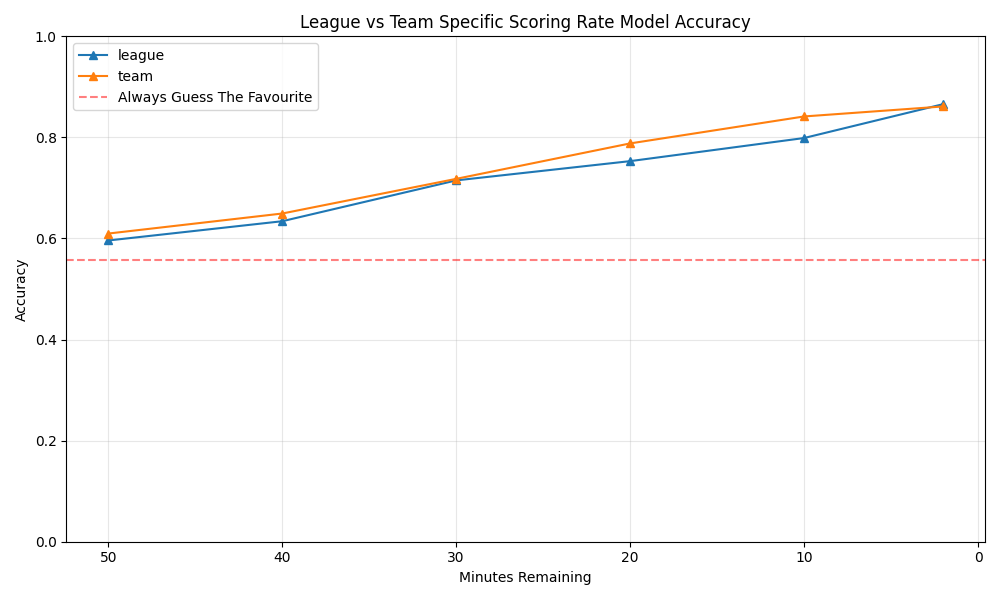
\includegraphics[width=\textwidth]{appendix/BvHAcc.png}
  \caption{League-wide vs Team-specific Model Accuracy.}
  \label{fig:bvhacc}
\end{figure}

\begin{figure}[h!]
  \centering
  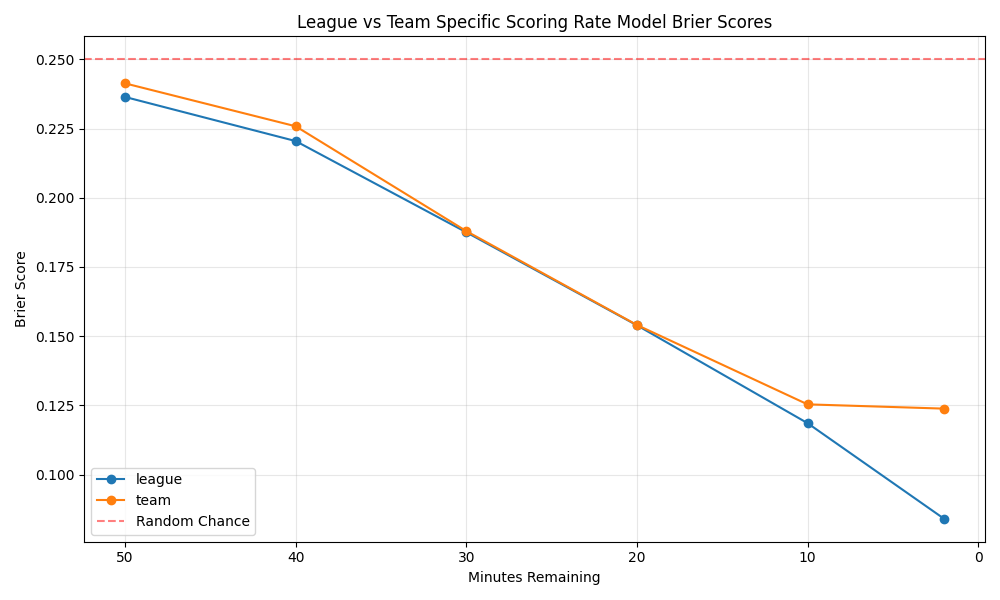
\includegraphics[width=\textwidth]{appendix/BvHBrierS.png}
  \caption{League-wide vs Team-specific Model Brier Score.}
  \label{fig:bvhb}
\end{figure}

\begin{figure}[h!]
  \centering
  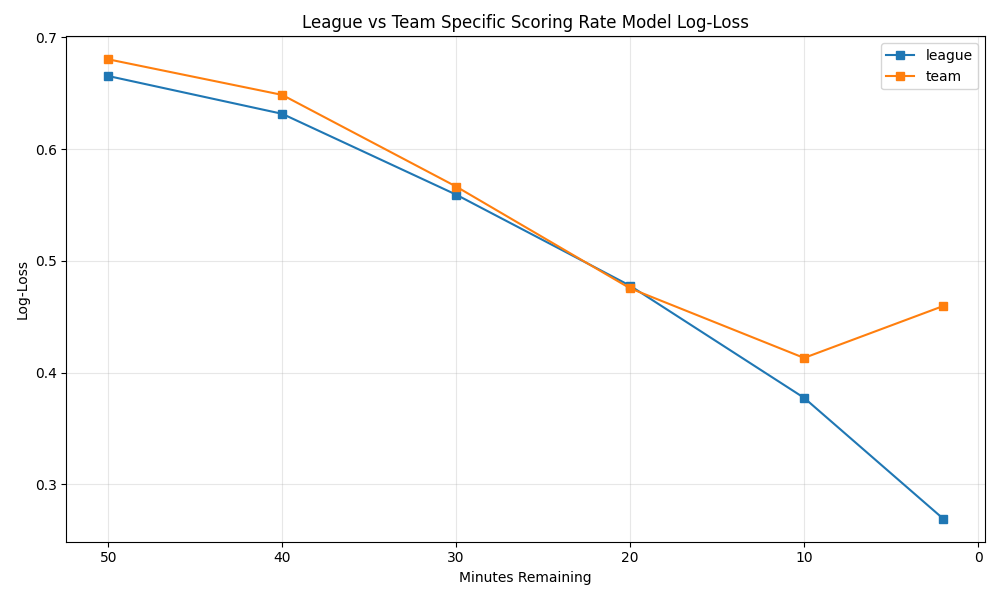
\includegraphics[width=\textwidth]{appendix/BvHLogLoss.png}
  \caption{League-wide vs Team-specific Model Log Loss.}
  \label{fig:bvhll}
\end{figure}

\begin{figure}[h!]
  \centering
  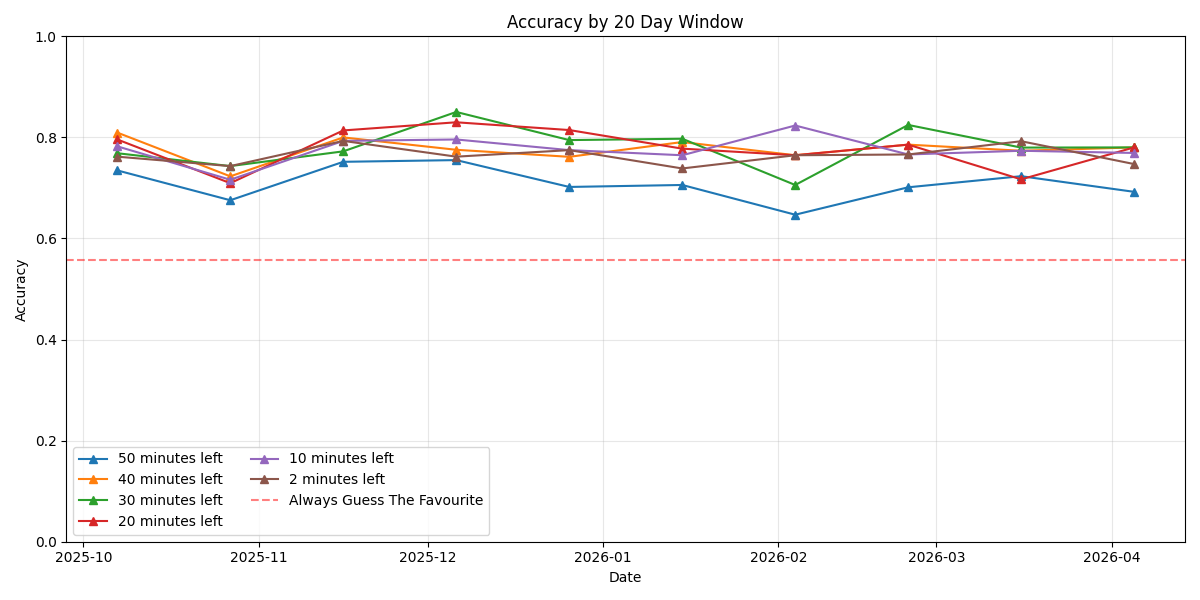
\includegraphics[width=\textwidth]{appendix/20DayAcc.png}
  \caption{20 Day Model Accuracy.}
  \label{fig:20acc}
\end{figure}

\begin{figure}[h!]
  \centering  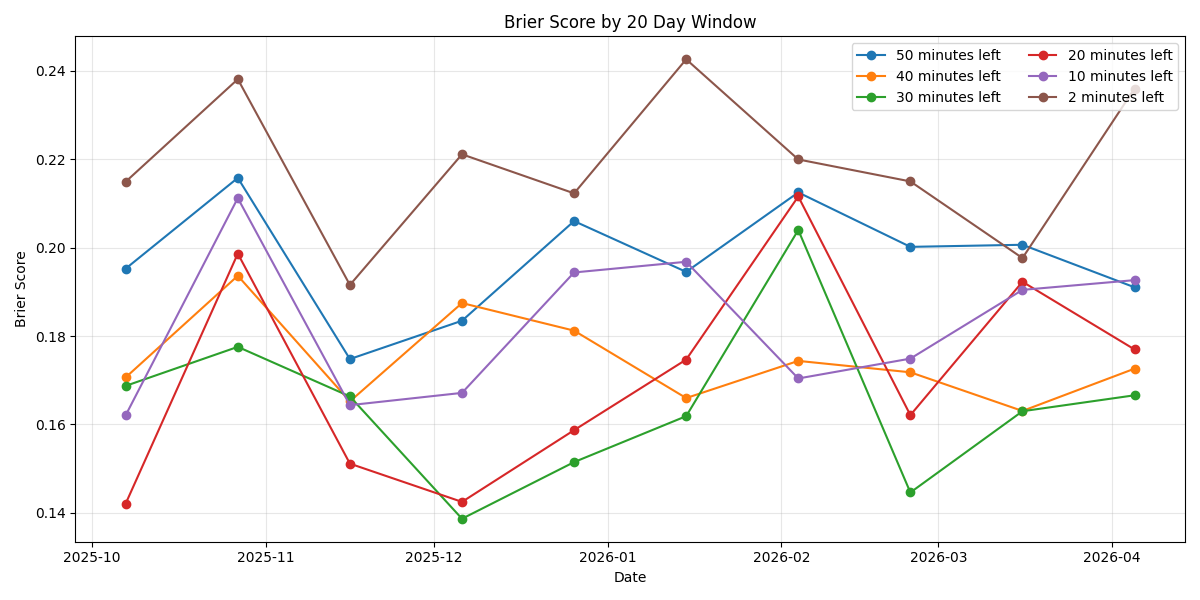
\includegraphics[width=\textwidth]{appendix/20DayBScores.png}
  \caption{20 Day Model Brier Score.}
  \label{fig:20bscore}
\end{figure}

\begin{figure}[h!]
  \centering
  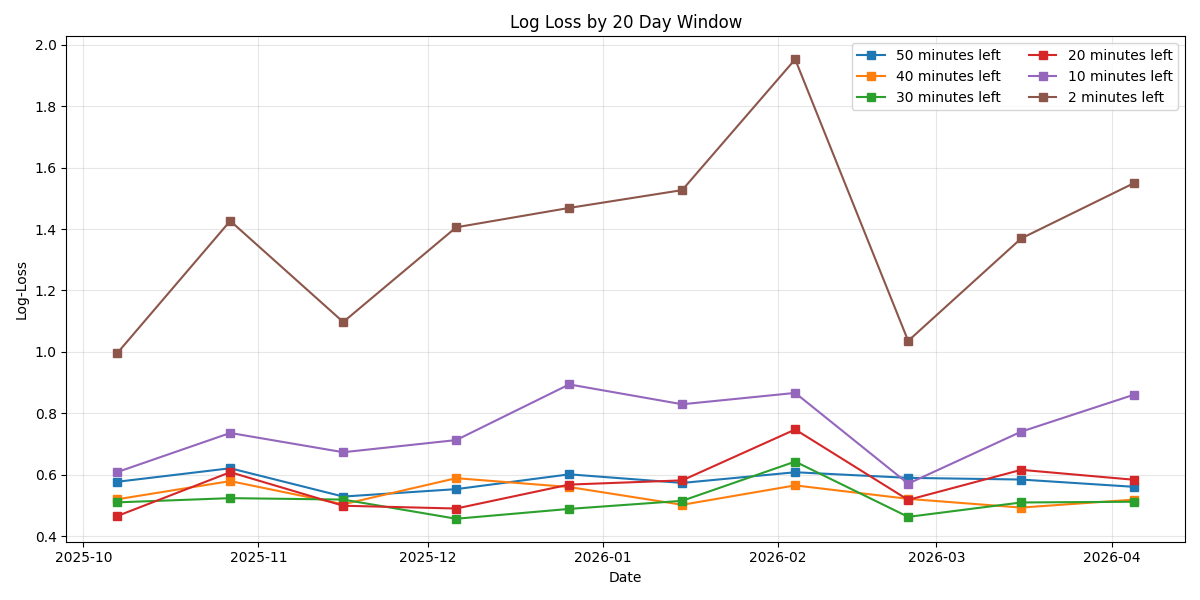
\includegraphics[width=\textwidth]{appendix/20DayLL.png}
  \caption{20 Day Model Log Loss.}
  \label{fig:20ll}
\end{figure}

\end{document}
